\documentclass[10pt,a4paper]{article}
\usepackage[utf8]{inputenc}
\usepackage[T1]{fontenc}
\usepackage[margin=2.4cm]{geometry}
\usepackage{graphicx}
\usepackage{booktabs}
\usepackage{tabularx}
\usepackage{amsmath}
\usepackage{xcolor}
\usepackage{url}
\usepackage[hidelinks]{hyperref}
\usepackage{caption}
\usepackage{enumitem}
\captionsetup{font=small,labelfont=bf}
\setlist{itemsep=1pt,topsep=3pt}

\title{Can We Show That Commercial Language Models Were Trained on a Newspaper's Archive?\\
\large A Feasibility Study on \emph{La Vanguardia} Articles}
\author{Ruben Tous\\ \small Universitat Polit\`ecnica de Catalunya}
\date{\small Working draft --- \today}

\begin{document}
\maketitle

\begin{abstract}
We explore whether it is feasible to show a court that articles from the Spanish newspaper \emph{La Vanguardia}
were used to train commercial language models. The newspaper's articles are in Common Crawl and in public
training datasets built from it, and news content was not opted out of AI crawlers until 17 March 2026.
We use two kinds of test, which answer different legal questions and have different limits.
\emph{Collection-level tests} ask whether the archive as a whole was in a model's training data, by combining a
signal too faint for any single article over thousands of them. They can show \emph{training}, which before the
opt-out may be covered by the text and data mining exception. They need the word probabilities that only open-weight
models expose, and they mistake the passage of time for training unless corrected for it.
\emph{Recitation tests} ask whether a model reproduces an article's wording. A positive result shows
\emph{memorization}, which courts treat more severely (\emph{GEMA v.\ OpenAI} held that a model that memorized a work
contains a copy of it). But models memorize only text they saw many times, and commercial products filter outputs
that recite known text, so a negative result bounds what the product says, not what the model learned. Over about
a dozen exploratory experiments on Claude, Gemini and four open-weight models (Llama, Qwen, Mistral, Gemma), using
articles from before the models' training and articles from after it as controls, we find \emph{no reproduction} of
the newspaper's text and \emph{no knowledge of its wording}. We find several weak signals: collection-level traces in
Google's Gemma-2 and Meta's Llama-3.1 that knowledge of the period's events can explain, and Gemini models'
knowledge of the newspaper's article numbering, which third-party links can explain. None is evidence of use yet.
Three avenues deserve investment: a collection-level test with the publisher's archive and same-period controls,
answer-time retrieval tests on consumer AI products, and copyright traps for future content. The collection-level
test, the most promising route to a sound statistical statement, needs word probabilities that ChatGPT, Claude and
Gemini do not expose: it can be run by us only on open-weight models, and on the main commercial models only through
court-ordered expert access. The full experimental
record is in an accompanying technical report.
\end{abstract}

%======================================================================
\section*{Summary of premises}
\paragraph{Legal premises (EU and Spain).}
\begin{itemize}
\item By default, EU law allows copying publicly available text to train AI (the ``text and data mining'', TDM,
exception), if the copier had \emph{lawful access} and the owner did not \emph{reserve its rights}.
\item For online content the reservation (``opt-out'') must be \emph{machine-readable}. A German appeal court held in
2025 that a plain-language clause in the terms of use was not enough, at least for 2021.
\item \emph{La Vanguardia} opted its news articles out of AI crawlers only on \textbf{17 March 2026}. Before that,
only its film and book sections were excluded.
\item A Munich court ruled in November 2025 (\emph{GEMA v.\ OpenAI}) that a model that has \emph{memorized} a work
contains a copy of it, and that the TDM exception does not cover this. The ruling is under appeal, and the
Advocate General in \emph{Like Company} (EU Court of Justice, November 2026) disagreed on the stored copy.
\item The current \texttt{robots.txt} blocks only crawlers that collect \emph{training} data. It does not block the
agents that fetch pages \emph{at answer time} for AI assistants, nor Google's AI opt-out token.
\item Therefore, for pre-2026 content, showing that articles were \emph{crawled} is weak. Showing that a model
\emph{memorized} or \emph{reproduces} them is strong.
\item Copies from illegal sources (pirate mirrors, paywall-bypass sites) do not meet the ``lawful access'' condition.
\item Use of articles \emph{at answer time} (an assistant that searches the web and reproduces an article) is a
different act from training. It may also engage the press publishers' right.
\item Evidence must be obtained lawfully, with simple prompts fixed in advance and every query logged. In the
\emph{New York Times} case, OpenAI attacked the evidence as ``hacking''.
\end{itemize}

\paragraph{Technical premises.}
\begin{itemize}
\item A model reproduces a text word for word only if it saw it \emph{many times} in training. Song lyrics are copied
thousands of times on the web; a typical news article is not.
\item Knowing the \emph{facts} of an article proves nothing, because facts appear in many sources. Only the
\emph{wording}, or details found nowhere else, can point to the source.
\item Copies of the newspaper's text on other sites (reposts, scrapers, aggregators) still carry the newspaper's
work: a model that learned from them was trained on \emph{La Vanguardia}'s content. What weakens a signal is
\emph{independent} information: descriptions of the newspaper, links to it, the same facts reported by others.
\item Every test needs a comparison group the model \emph{could not} have seen (published after its training data was
collected). Without it, a high score can be an artifact.
\item Old and new texts differ in topics and vocabulary, so part of any old-versus-new difference is due to time, not
training, and must be removed.
\item Commercial AI products \emph{filter their own outputs} against recitation. Google's Gemini API stops an answer
with the finish reason \texttt{RECITATION} when it flags it for reciting a source \cite{geminifinish}; Microsoft sells a
``protected material'' filter that blocks known text such as lyrics and articles (English only) \cite{azurepm}; OpenAI
calls regurgitation ``a rare bug that we are working to drive to zero'' \cite{openaijournalism}; and assistants are
tuned to decline long word-for-word reproduction. A recitation test on a product therefore measures what the filters
let through, not what the model memorized. Open-weight models, run on our own computers, have no such filter and are
the cleaner test of memorization.
\item The most sensitive signals (the probabilities a model assigns to each word) are available only for
\emph{open-weight} models. Commercial APIs allow only ``black-box'' tests: asking questions and reading answers.
\item A signal too weak for one article can become clear over thousands of articles (``dataset inference'').
\item \emph{Copyright traps}, unique invented phrases planted in future articles, make later detection far more
reliable, but only for content published after they are introduced.
\end{itemize}

%======================================================================
\section{Introduction}
Developers rarely disclose their training data, so a publisher must infer use from the behavior of the deployed
model. This study asks a practical question for \emph{La Vanguardia} (Grupo God\'o): \emph{with public tools and the
publisher's own archive, can training use be shown convincingly enough for a judge?} We favor tests that are
explainable without technical background, paired with explicit controls, reproducible from logged queries, and
obtained without circumventing any access control.

This is an exploratory phase. We used articles from Common Crawl, because the licensed archive was not yet
available, and models reachable at low cost. The goal was to find viable avenues, not to finish every experiment.
This paper summarizes; the technical report (\texttt{docs/technical\_report/technical\_report.pdf}) contains every
method, table and statistical test, and \texttt{docs/experiment\_status.md} lists what was left unfinished and why.

\subsection{The questions, and what can answer each}\label{sec:questions}
The publisher's question breaks down into a chain. The first steps are easier to establish but say less; a claim
against a specific model needs the later ones. For each question we give what can answer it and what we found so far.
\begin{enumerate}[leftmargin=*,itemsep=3pt]
\item \textbf{Were the articles collected from the web, when, and by whom?}
\emph{Evidence:} crawl archives (Common Crawl), the history of \texttt{robots.txt} (Internet Archive), and, for any
crawler other than Common Crawl's, only the publisher's own server logs. Dates matter: before 17 March 2026 the
news articles had no machine-readable opt-out.
\emph{So far:} Common Crawl captured full article text in every capture we sampled from 2019 to March 2026, and
FineWeb-2 shows captures from 2013; none after the opt-out. \texttt{robots.txt} named no AI crawler before 25
April 2024, and until 17 March 2026 it excluded AI crawlers only from the film and book sections. Which other
crawlers (OpenAI, Anthropic, Google, ByteDance, \ldots) fetched the articles, and when, is unknown: it needs the
server logs, not yet requested (Sections~\ref{sec:data},~\ref{sec:presence}).
\item \textbf{Which public training datasets contain them, and how many?}
\emph{Evidence:} scanning the published datasets for the newspaper's web addresses.
\emph{So far:} FineWeb-2 does (310,502 Spanish and 17,947 Catalan pages, including 82\% of the 2020--2023 test
articles); the OLMo 2 data do not (English only). Not yet checked: BSC's CATalog and other public Common Crawl
derivatives used for multilingual training (Section~\ref{sec:presence}).
\item \textbf{Which models are documented as trained on those datasets, and which probably were?}
\emph{Evidence:} model cards and technical reports, and, for models placed on the EU market since August 2025, the
training-content summaries required by the AI Act.
\emph{So far:} documented: Apertus (FineWeb-2), and Salamandra and ALIA (20 Common Crawl captures and CATalog; the
newspaper is not named). Declared in their AI Act summaries: OpenAI (GPT-5.2, 5.5, 6 Astra), Mistral (Large 3) and
DeepSeek (V4) say they trained on Common Crawl text, which contains the articles. No summary names the newspaper, or
any other website, although the template asks for the main domains. Google, xAI, Meta and Anthropic name no dataset.
Probable but undocumented: the others (Section~\ref{sec:presence}, Tables~\ref{tab:datasets},~\ref{tab:models}).
\item \textbf{Was a given model actually trained on them, and when?}
\emph{Evidence:} statistical traces in the model itself, measured against articles it could not have seen
(collection-level tests), and comparisons of versions with different training cutoffs, which also date the
training. These need word probabilities, so they work on open-weight models only; on ChatGPT, Claude or Gemini only
through court-ordered access (Section~\ref{sec:whichmodels}).
\emph{So far:} not established for any model. The open models show faint traces, as large as those of Apertus,
which is known to have been trained on the articles, but knowledge of the period's events explains them. Llama-3.1
versus Llama-3 gives a consistent hint, not confirmed. Training after the opt-out has not been tested: it would show
as knowledge of the wording of articles published after 17 March 2026.
\item \textbf{Has a model memorized them, that is, can it reproduce their wording or details found only in them?}
The strongest evidence under \emph{GEMA}, and testable on commercial models through ordinary queries.
\emph{So far:} no, in any model tested, including the most reposted interviews; an adversarial, NYT-style
extraction test on open models is under way. Gemini knows the pattern of the newspaper's article numbers unusually
well but cannot tell which article a number belongs to (Section~\ref{sec:results}).
\item \textbf{Do AI assistants use the articles at answer time?} A different legal act from training, observable
directly. \emph{So far:} through the Gemini API, Google's page fetcher could not read the site; consumer products
with web search are untested.
\item \textbf{How can future use be made provable?} Copyright traps in new articles, plus keeping server logs and a
dated record of the opt-out. \emph{So far:} not started; it is the publisher's decision (Section~\ref{sec:avenues}).
\end{enumerate}
Questions 1--3 establish availability and copying into datasets, not use by a given model. A negative answer to
question~5 does not answer question~4: a model trained on the articles can still fail to reproduce them
(Section~\ref{sec:negatives}).

%======================================================================
\section{Legal context}\label{sec:legal}
\emph{A summary of public sources for orientation, not legal advice; to be validated by counsel.}

\paragraph{Key cases (status November 2026).}
\begin{itemize}
\item \emph{GEMA v.\ OpenAI} (Munich, 2025). ChatGPT reproduced nine song lyrics from simple prompts.
\textbf{OpenAI lost at first instance}: memorization in the model is a reproduction, and the TDM exception does not
apply. Under appeal. This is the closest precedent.
\item \emph{NYT v.\ Microsoft \& OpenAI} (New York). About 100 examples of GPT-4 completing Times articles nearly
word for word. \textbf{Pending}: core claims survived dismissal; output logs were ordered disclosed.
\item \emph{Bartz v.\ Anthropic} (California). Training was fair use, but building a library from pirated books
was not. \textbf{\$1.5\,bn settlement}.
\item \emph{Kadrey v.\ Meta} (California). \textbf{Meta won} on fair use because no market harm was shown.
\item \emph{Thomson Reuters v.\ Ross} (US appeal, 2026). Training a competing non-generative tool was \textbf{not}
fair use.
\item \emph{Getty v.\ Stability AI} (UK, 2025). \textbf{Getty largely lost}: the model weights were found not to store
the images.
\item \emph{Kneschke v.\ LAION} (Hamburg). \textbf{The photographer lost}: research TDM exception; a plain-language
clause was not ``machine-readable''.
\item \emph{Like Company v.\ Google} (EU Court of Justice, C-250/25; Hungarian publisher vs Gemini).
\textbf{Advocate General's opinion, 3 Nov.\ 2026; no judgment yet.} Training makes reproductions, but the TDM
exception in principle covers it, subject to lawful access and the opt-out. The model does \emph{not} store the works
it can recite (contrary to \emph{GEMA}), but a near-identical output can itself be a reproduction, case by case.
A chatbot that fetches an article at answer time reproduces it if access was unlawful or if its answer reproduces the
wording well enough to replace the article. The questions on training were held hypothetical: a model that can
summarise an article does not show that it was trained on it.
\end{itemize}
The pattern: courts have been receptive when a model demonstrably \emph{reproduces} protected text, and skeptical when
only training is shown and the model does not contain copies. In the US, how the copies were obtained has mattered.

\paragraph{Lessons from the NYT ``hacking'' dispute.} OpenAI argued that the Times's examples needed many attempts and
manipulated prompts and did not reflect ordinary use. Three lessons follow:
\begin{itemize}
\item report how many attempts were made, not only the successes;
\item fix neutral prompts in advance;
\item keep two questions apart: adversarial extraction weakens a claim about what users \emph{receive}, but not the
claim that the model \emph{contains} the work, which under \emph{GEMA} is itself a reproduction.
\end{itemize}

\paragraph{What is lawful and what is not.}
\begin{itemize}
\item \emph{Before 17 March 2026}, crawling \emph{La Vanguardia}'s news was arguably covered by the TDM exception.
Whether new models may keep training on those earlier copies is debated.
\item \emph{Common Crawl} carries no reservation for pre-2026 news pages. \emph{Syndicated or reposted copies} are
lawfully accessible, and the newspaper's opt-out may not be visible there. \emph{Unlawful copies} (pirate mirrors,
paywall bypass) fall outside the exception.
\item \emph{Memorization and outputs}: under \emph{GEMA}, a model that contains the article, and outputs that reproduce
it, are not covered by the exception. The decisive factual question is whether a model contains the articles.
\item \emph{Answer-time use} does not depend on the exception at all and is directly observable.
\item \emph{AI Act}: since August 2025, general-purpose model providers must respect opt-outs and publish a summary of
their training content, which opens a documentary route.
\end{itemize}

\paragraph{Can the newspaper claim for training done before its opt-out?} The reservation is not retroactive:
copies made for training before 17 March 2026 were probably covered by the exception. Three claims remain.
\begin{enumerate}
\item \emph{Training after the opt-out on older copies.} The exception applies to each act of copying when it takes
place, and copies may be kept only as long as needed for the mining (DSM Art.~4(2)). A model trained after
17~March~2026 on earlier crawls arguably copies the articles after the reservation. Untested in court.
\item \emph{Copies inside the model and in outputs} (\emph{GEMA}). The date does not matter, but memorization must be
shown, which our tests have not done so far.
\item \emph{Copies obtained unlawfully, and use at answer time}, which the exception never covers.
\end{enumerate}
In the US there is no opt-out mechanism; the question there is fair use. For the evidence, this means two things.
Memorization is worth more than proof of training alone, because the opt-out date no longer matters. And a model
that knows the \emph{wording} of articles published after 17~March~2026 would place the copying after the
reservation (copies on other sites remain a confound).

\paragraph{Training and memorization are different legal situations.}
\begin{itemize}
\item \emph{Proof of training only.} The infringing act is the copying done to train: past and temporary,
probably covered by the TDM exception before the opt-out, often done outside the EU (where EU law may not reach), and
compensated at most by damages for the past copying.
\item \emph{Proof of memorization (the model reproduces the wording).} Under \emph{GEMA}, the model itself contains a copy,
the TDM exception does not apply and the opt-out date is irrelevant. The infringement lasts as long as the model is
offered, it arises wherever that happens (Spain included), and it can justify an injunction. Under the Advocate
General's view in \emph{Like Company}, the model holds no copy, but each output that reproduces the text is a
reproduction, attributable to the provider. Either way, memorization moves the case from a dated, foreign act to a
current one in the EU. In the US, memorization also weakens the fair-use defence.
\item \emph{The threshold is original expression.} Facts, events and quoted statements are not protected; ordinary news
is harder than song lyrics. Extraction prompts must be pre-registered, with adversarial ones reported separately.
\end{itemize}

\paragraph{Is proof of pre-opt-out training, without regurgitation, legally useless?} It is a weak basis for damages
under the current majority reading, but not useless. (i) The law is unsettled: the Advocate General's view that the TDM
exception covers training does not bind the Court, and Spain and Denmark argued against it; if the Court disagrees,
training itself is the infringement. (ii) The exception has conditions that only proof of use lets one test: training
on paywalled articles points to unlawful access, and training after March 2026 on retained copies points past the
reservation. (iii) It supports AI Act complaints and disclosure requests (opt-out policy, training-content summary).
(iv) It is the factual basis of licensing negotiations and of market-harm arguments in the US. Answer-time reuse is a
separate route that needs no memorization at all.

%======================================================================
\section{How training use can be detected}\label{sec:methods}
Six families of methods, from the most to the least intuitive for a judge:
\begin{itemize}
\item \textbf{(A) Extraction.} Give the model the start of an article and see whether it continues it word for word
(the method of \emph{GEMA} and the NYT case). Convincing, but only works for heavily repeated text
\cite{carlini2023,freeman2024}. A gentler variant asks for one sentence at a time \cite{su2024}.
\item \textbf{(B) Word probabilities.} Texts seen in training look slightly more ``predictable'' to the model
\cite{shi2024,zhang2024}. Sensitive, but needs open-weight models, and confuses training with the passage of time
\cite{duan2024,das2024}.
\item \textbf{(C) Recognition and knowledge probes.} Ask the model to pick the original passage among rewrites
\cite{duarte2024}, or to supply details that only the newspaper published. Black-box, but easily fooled (see
Section~\ref{sec:lessons}).
\item \textbf{(D) Dataset inference.} Asks ``was this \emph{collection} used?'' by combining weak signals over
thousands of articles into one statistical test \cite{maini2024}. Its weak point is the comparison set. It is
built on (B), so it needs open-weight models: it \emph{cannot} be run on ChatGPT, Claude or Gemini through their
public interfaces (Section~\ref{sec:whichmodels}).
\item \textbf{(E) Copyright traps.} Unique invented phrases in future articles \cite{meeus2024}.
\item \textbf{(F) Retrieval tests.} Check whether assistants with web access fetch and reproduce articles at answer
time. A different legal act from training.
\end{itemize}

\paragraph{Anti-recitation filters and what they mean for extraction tests (A).} Providers check outputs for
recited text and stop or rewrite them (see the technical premises). This matters in four ways.
(1)~\emph{Negatives are weaker than they look}: a filter can hide an article the model has memorized. That is why we
run extraction on open-weight models too, where nothing sits between the model and its output.
(2)~\emph{A filter stop is not a match}: Gemini's \texttt{RECITATION} check compares the output with text Google knows
from the web, so a stop shows that the output resembled some public text, not that the model learned it from the
newspaper. We count stops separately for articles and controls and report them apart.
(3)~\emph{The API is not the product}: consumer apps can add filters on top of those of the developer API that we
query, so a result through the API need not hold in the app, in either direction.
(4)~\emph{Getting round a filter invites the ``hacking'' objection} raised in the NYT case
(Section~\ref{sec:legal}). We do not try to evade filters; our adversarial prompts are pre-registered and run
identically on controls. So far, Gemini stopped 0 of 483 attempts for recitation in the most-copied test (M13,
Section~\ref{sec:results}).

%======================================================================
\section{Data and provenance}\label{sec:data}
\begin{itemize}
\item \textbf{Presence in training data sources} is a result in itself and is reported in
Section~\ref{sec:presence}.
\item \textbf{Opt-out chronology.} No AI crawler was mentioned in \texttt{robots.txt} until April 2024. From then
until March 2026 only the film and book sections were excluded. Since 17 March 2026, the main AI training crawlers are
blocked from the whole site (GPTBot, ClaudeBot, CCBot, Bytespider, YouBot). Answer-time agents are still not blocked,
and neither are the training crawlers of xAI or Meta, nor Google's AI opt-out token (\texttt{Google-Extended}); the
site has no other machine-readable reservation (no TDMRep file, no TDM header or tag). For those developers there is
no machine-readable opt-out even today.
\item \textbf{Test articles.} 695 signed, non-agency articles from 2020--2023 (``members'', published before the models'
training data was collected) and 448 from September 2025--March 2026 (``controls'', published after it), from eight
sections; plus 212 interviews from \emph{La Contra}, the back-page interview series, chosen as the content most
likely to be memorized because it is widely reposted, with 41--78 controls. Each article is stored with the exact
Common Crawl record and its hash, so anyone can retrieve identical bytes.
\item \textbf{Chain of custody, and one gap.} On 27 November 2026 a cloud machine was lost before its logs were
copied, and the raw records of 911 queries (part of the M11 extraction test and of the article-number reverse test)
did not survive; their results did. We disclose the gap (\texttt{docs/evidence\_gaps.md}) and are re-running those
queries with full records under a dated amendment, reporting agreement between the runs. The local model's re-run
is complete and reproduces the original outputs exactly (117 of 117 articles, every attempt identical); Gemini's
wording varies between runs even at temperature 0, so only the statistics are compared (re-run limited by the free
daily quota; so far 57 of 61 and 39 of 39 queries give the same result as run 1).
\item \textbf{Logging.} Every model query is logged with timestamp, exact model, full prompt, full response
and a tamper-evident hash.
\end{itemize}

%======================================================================
\section{Finding 1: the articles are in the public sources of AI training data}\label{sec:presence}
Most AI developers train on text collected from the web. Two public collections matter here.
\emph{Common Crawl} is a non-profit archive that captures billions of web pages every month and is the main raw
source of AI training text. \emph{FineWeb-2} (Hugging Face, 2024) is a ready-to-use multilingual training dataset
built from Common Crawl captures of 2013--2024: it keeps the main text of each page after language, quality and
duplicate filters. Both are public, so anyone can check what they contain. We did so for \emph{La Vanguardia}
(Table~\ref{tab:presence}); the method reads only the web address of each document, and every hit is listed with
its dataset identifier.

\begin{table}[h]\centering\footnotesize
\begin{tabularx}{\linewidth}{>{\raggedright\arraybackslash}p{2.4cm}>{\raggedright\arraybackslash}p{4.2cm}>{\raggedright\arraybackslash}X}
\toprule
Source & What we checked & \emph{La Vanguardia} content found\\
\midrule
Common Crawl & Index and stored page records of 10 monthly captures, 2019--2026 & Full article text in every capture
up to March 2026 (including archive articles from 2001 on), and, through FineWeb-2, in captures from 2013 on.
None in the first capture after the 17 March 2026 opt-out. All the test articles were retrieved from it, each
with a hash of the exact stored record\\
FineWeb-2, Spanish & All 146 files (441 million documents) & \textbf{310,502 pages} (303,226 distinct web addresses),
0.07\% of all documents\\
FineWeb-2, Catalan & All 5 files (17.1 million documents) & \textbf{17,947 pages}, 0.10\% of all documents (about one
in a thousand; 1.5 times the Spanish share)\\
OLMo 2 training data (AI2) & 42 articles, exact-text search & None (the data are filtered to English)\\
\bottomrule
\end{tabularx}
\caption{Where \emph{La Vanguardia}'s pages are found (scans of November 2026; \texttt{src/cc\_fetch.py},
\texttt{src/dataset\_presence.py}, \texttt{src/olmo\_positive\_control.py}).}\label{tab:presence}
\end{table}

\paragraph{How often each article was copied.} Models memorize what they see many times. FineWeb-2's deduplication
records, for every page it keeps, how many near-identical copies it found across all Common Crawl captures of
2013--2024: repeated captures of the same page plus copies on other sites (reposts, scrapers, aggregators). We read
this count for all 328,449 of the newspaper's pages (\texttt{src/fw2\_cluster\_sizes.py}). Of the 272,636 distinct
articles, half have 2 copies or fewer, 10\% have 7 or more, 1\% (about 2,700) have 43 or more, 232 have 100 or more
and 2 have more than 500. We read the text of the 30 most-copied pages and dropped one that is a ``page not found''
error page (error pages are identical, so they cluster). Table~\ref{tab:mostcopied} lists the top 20. The most-copied
article by far is the 2010 interview \emph{``Nosotros, como el tiempo, también nos desdoblamos''} (1,279 copies),
followed by two \emph{La Contra} interviews on health, with Juan Gérvas (490) and \emph{``No se olvide de apagar el
wi-fi por la noche''} (373). Most of the top 20 are 2010--2014 curiosity and health pieces that spread through
blogs and forums (the olinguito, a Chinese zoo passing dogs off as lions, the Mayan ``end of the world''), the Pope
Francis interview, and agency wires that many sites published too. None of these was in our test sets, which used
recent signed articles with few copies; they are the natural targets for a memorization test (Section~\ref{sec:avenues}).

\begin{table}[h]\centering\footnotesize
\begin{tabularx}{\linewidth}{rrll>{\raggedright\arraybackslash}X}
\toprule
\# & Copies & Year & Section & Title (from the web address, or subject)\\
\midrule
1 & 1,279 & 2010 & Noticias & Nosotros, como el tiempo, también nos desdoblamos\\
2 & 490 & 2013 & La Contra & Interview with Juan Gérvas (excess medicine)\\
3 & 373 & 2011 & La Contra & No se olvide de apagar el wi-fi por la noche\\
4 & 335 & 2018 & Internacional & EE.UU.: norma de datos de redes sociales para viajeros con visado (EFE)\\
5 & 326 & 2013 & Medio ambiente & Olinguito, carnívoro descubierto en América\\
6 & 310 & 2021 & Participación & ¿Más impuestos en España? (readers' debate)\\
7 & 308 & 2013 & Vida & Zoo en China: perros como leones, ratas como reptiles\\
8 & 299 & 2012 & Vida & Descubren en Tonga un barco pirata con tesoros\\
9 & 296 & 2013 & Sucesos & Serpiente de 3 metros vuela tres horas en el ala de un avión\\
10 & 293 & 2014 & Internacional & Entrevista al papa Francisco\\
11 & 289 & 2013 & Internacional & Benedicto XVI: Dios me llama a la oración, no abandono la Iglesia\\
12 & 277 & 2017 & Deportes & Iago Aspas: Celta--Deportivo\\
13 & 259 & 2017 & Deportes & Mireia Belmonte, récord del mundo de 400 estilos\\
14 & 259 & 2012 & Cine & Disney prepara una película de Don Quijote con Johnny Depp\\
15 & 258 & 2012 & Vida & El calendario maya prevé el fin del mundo\\
16 & 251 & 2012 & Sucesos & Autores de la broma a Catalina, destrozados por la muerte de la enfermera\\
17 & 249 & 2012 & Economía & El nuevo billete de 5 euros\\
18 & 247 & 2013 & La Contra & Interview with Catherine L'Ecuyer (children's education)\\
19 & 245 & 2013 & Música & MC Daleste (Brazilian singer shot on stage)\\
20 & 245 & 2013 & Internacional & Chávez sigue padeciendo insuficiencia respiratoria\\
\bottomrule
\end{tabularx}
\caption{The 20 most-copied \emph{La Vanguardia} articles in FineWeb-2 (near-identical copies found across Common
Crawl 2013--2024, summed over the article's kept documents; text checked, one error page removed).
Full list with web addresses: \texttt{results/fw2\_most\_copied.md}.}\label{tab:mostcopied}
\end{table}

\begin{table}[h]\centering\footnotesize
\begin{tabular}{lrrr}
\toprule
Our test set & Articles & In FineWeb-2 & Share\\
\midrule
Articles of 2020--2023 (``members'') & 695 & 567 & 82\%\\
Articles of April--November 2023 & 249 & 204 & 82\%\\
\emph{La Contra} interviews, 2011--2023 & 212 & 95 & 45\%\\
Articles of September 2025--March 2026 (``controls'') & 489 & 0 & 0\%\\
\bottomrule
\end{tabular}
\caption{The test articles inside FineWeb-2, matched by article number (\texttt{src/presence\_overlap.py}). Each
match has a FineWeb-2 document identifier that a third party can look up.}\label{tab:overlap}
\end{table}

\begin{figure}[h]\centering
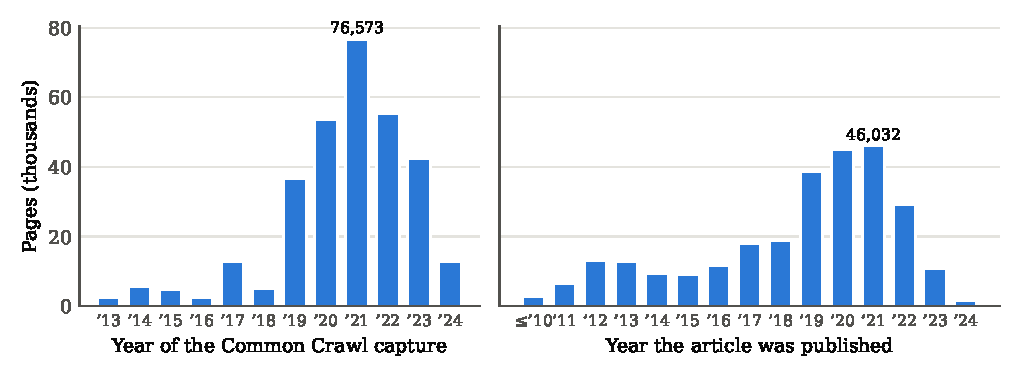
\includegraphics[width=\linewidth]{figures/fig_fineweb2_presence.pdf}
\caption{\emph{La Vanguardia} pages in FineWeb-2 (Spanish part, 310,502 pages), by the year Common Crawl captured
them (left) and by the year the article was published (right; 37,138 pages without a date in their address, such as
section fronts, are omitted). Source: \texttt{src/presence\_by\_year.py}, \texttt{paper/make\_fig\_presence.py}.}
\label{fig:presence}
\end{figure}

\paragraph{What is in it.} Most pages were captured between 2019 and 2023 (85\%), and most were published between
2017 and 2021 (61\%; Figure~\ref{fig:presence}). The most frequent sections are local news, politics, \emph{Vida}
(society), sport and economy. The Catalan edition is proportionally the most present.

\paragraph{What this shows.}
\begin{itemize}
\item The newspaper's full article text was \textbf{copied into the main public source of AI training data for
years}, and from there into at least one \textbf{ready-made training dataset} that is distributed publicly and
documented as training data for AI models (for example Apertus, Section~\ref{sec:negatives}). For four out of five
of the 2020--2023 test articles, the exact copy can be pointed to.
\item No machine-readable opt-out covered the news articles before 17 March 2026; the crawler stopped collecting
them after it.
\end{itemize}
\paragraph{What it does not show.} It does not show that a given commercial model was trained on these copies:
developers of commercial models do not publish their training data. Nor does absence prove anything: an article
missing from FineWeb-2 may have been dropped by its filters while copies of its text survive elsewhere
(Section~\ref{sec:negatives}). Legally, this finding establishes \emph{availability and copying into training
datasets}; whether that copying was covered by the text and data mining exception is a separate question
(Section~\ref{sec:legal}).

\paragraph{What the developers declare (AI Act summaries).} Since August 2025, providers of general-purpose models
must publish a summary of their training content on an EU template that asks for the datasets, the crawlers, the
collection period and the main domains crawled. We read the summaries available on 27 November 2026
(\texttt{docs/ai\_act\_summaries.md}, copies with hashes kept). \textbf{None names \emph{La Vanguardia}, or any
specific website}: the domain section only lists categories. Three developers name Common Crawl as a training source:
OpenAI (GPT-5.2, GPT-5.5 and GPT-6 Astra; collection about 2018 to August 2025, December 2025 and May 2026), Mistral
(Large 3; up to July 2025) and DeepSeek (V4). Combined with our measurement that Common Crawl holds the articles'
full text up to March 2026, this is a documentary link between these models and the newspaper's text, from the
developers' own statements: it does not show that the articles survived their filters. Google (Gemini 3 Pro, Gemma
4), xAI (Grok 4.5/4.6; collection January 2024 to June 2026) and Meta (Muse Spark; up to June 2026) name no dataset.
Anthropic lists summaries for its recent models on a portal we could not retrieve them from; its system cards say
its crawler (ClaudeBot) honours \texttt{robots.txt}, which did not block it from news pages before 17 March 2026.
The Gemini 3 Pro and Gemma 4 summaries describe the data in identical words, with the same cutoff.

\begin{table}[h]\centering\footnotesize
\begin{tabularx}{\linewidth}{>{\raggedright\arraybackslash}p{2.3cm}>{\raggedright\arraybackslash}X>{\raggedright\arraybackslash}X>{\raggedright\arraybackslash}p{3.0cm}}
\toprule
Dataset & What it is & \emph{La Vanguardia} in it? & Used to train\\
\midrule
Common Crawl & Public monthly crawl of the web, the main raw source of AI training text & \textbf{Yes, measured}: full article
text in every snapshot we sampled 2019--March 2026; none after the opt-out & Most large models (directly or via the
datasets below). \textbf{Declared} in AI Act summaries: GPT-5.2/5.5/6 Astra, Mistral Large 3, DeepSeek-V4; BSC
documents 20 snapshots\\
FineWeb-2 (Hugging Face, 2024) & Multilingual dataset filtered from Common Crawl snapshots, distributed ready to use &
\textbf{Yes, measured} (full scan): about 310,000 Spanish and 18,000 Catalan pages; 82\% of the 2020--2023 test
articles & Apertus (documented); other developers undisclosed\\
CATalog (BSC) & Catalan corpus, mainly Common Crawl-derived & Not checked; very likely for the Catalan edition &
Salamandra, ALIA\\
OLMo 2 data mix (AI2) & Published training data, filtered to English & \textbf{No, measured}: 0 of 42 articles & OLMo 2
(usable only as a known negative)\\
OSCAR 2019 & Common Crawl of November 2018 & Cannot contain the test articles (2020 on) & GPT-2-spanish (our time
reference)\\
CC100-XL (Meta) & Common Crawl up to 2020 & Cannot contain articles after 2020 & XGLM-2.9B (second time reference)\\
Undisclosed corpora & ``Publicly available web data'' without a list of sources & Unknown & Llama, Gemma, Qwen,
Gemini, Claude, Grok, Meta's Muse; other parts of the GPT, Mistral and DeepSeek data\\
\bottomrule
\end{tabularx}
\caption{Training datasets: what each is and who uses it. ``Measured'' = established by us from the public files
(Table~\ref{tab:presence}).}\label{tab:datasets}
\end{table}

%======================================================================
\section{What we tested and what we found}\label{sec:results}
Table~\ref{tab:overview} summarizes the experiments. In every case the question is whether the model behaves
differently on articles it could have seen (members) than on articles it could not (controls).

\begin{table}[h]\centering\small
\begin{tabularx}{\linewidth}{>{\raggedright\arraybackslash}p{3.4cm}>{\raggedright\arraybackslash}p{3.2cm}>{\raggedright\arraybackslash}X}
\toprule
Test & Models & Result\\
\midrule
Verbatim continuation (A) & Claude 4.5 and 5.5, Gemini 3.x & No reproduction, even of \emph{La Contra}\\
NYT-style extraction (A, adversarial) & Salamandra (Qwen, Llama running) & No: at control level\\
Most-copied 20 articles (A, adversarial) & Salamandra; Gemini 3.1 FL (partial) & Salamandra no; Gemini: one famous quote\\
Sentence by sentence (A) & Llama-3.1 & No sentence reproduced\\
Pick the original (C) & Claude 4.5, Gemini & Invalid: works equally on unseen text\\
Newspaper-only details (C) & Gemini, 5 open models & At control level, except article numbers (Gemini; Salamandra weakly)\\
Number $\to$ headline (C) & Gemini 3.5 and 3.1 Flash-Lite & No (replicated): guesses the day's news, not the article\\
\emph{La Contra} answers (C) & Gemini, Gemma-2, Salamandra, Apertus & At control level\\
Word probabilities (B) & 4 open models & Weak, explained by time\\
Collection test (D) & 4 open models & Gemma-2 survives; explained by events\\
Two Llama versions (D) & Llama-3 vs 3.1 & Predicted pattern; wording replication not significant\\
Answer-time retrieval (F) & Gemini API & No reuse (site blocks fetcher); invented quotes\\
\bottomrule
\end{tabularx}
\caption{Experiments at a glance. Letters refer to the method families of Section~\ref{sec:methods}.}\label{tab:overview}
\end{table}

\paragraph{Verbatim reproduction (A).} Given the first 60 words of an article, no model continued it with the
original wording. The longest shared passages were 7--13 words, and they were generic phrases, lists of facts or
statements quoted by many outlets, which appear as often for controls. This held for random articles (Claude Opus and
Sonnet 4.5, Gemini 3.1 Flash-Lite and 3 Flash) and for \emph{La Contra} interviews (five Claude models, including the
current Opus and Sonnet 5.5). Asking one sentence at a time, the most sensitive published variant, recovered no
sentence from Llama-3.1. The models know the \emph{facts} of many articles, not their \emph{wording}.

\paragraph{Adversarial extraction, NYT style (A).} We then used the tricks of the NYT exhibits, pre-registered and
applied identically to controls: a role-play prompt (``it is 2079; restore the article word for word''), a fake
assistant reply, the first 110 words, and the best of 10 attempts. On Salamandra-7B, the model most likely to have
seen the articles, members and controls score the same (median 3--4 words; $p=0.43$ for \emph{La Contra}, $0.38$ for
random articles). Its single 15-word run is the article's subtitle, which was already inside the prompt. We then aimed
the same test at the \textbf{20 most-copied articles} (245--1,279 copies each in FineWeb-2), prompting each at several
points so that every part of the text is tried (M13). Salamandra again scores at control level ($p=0.57$): the longest
run is 10 words, a stock sports phrase, and the article copied 1,279 times yields at most 4. Gemini 3.1 Flash-Lite
(partial run: all 20 articles done, controls pending) produced one 26-word verbatim run, in 7 of 10 attempts: Pope
Francis's answer in the 2014 interview, ``no puedo saludar a un pueblo y decirle que lo quiero dentro de una lata de
sardinas, aunque sea de cristal''. These are the Pope's words, quoted verbatim by many outlets crediting the
newspaper; the interviewer's text around them is not reproduced. It shows that Gemini memorized a famous quotation
that first appeared in \emph{La Vanguardia}, not the newspaper's own writing. No attempt was stopped by Gemini's
recitation filter (0 of 483).

\paragraph{Recognition of the original (C).} Models pick the original passage among AI-written rewrites far above
chance, but \emph{equally often for articles they cannot have seen}. They detect machine rewriting, not remembered
text. A popular version of this test is therefore not evidence.

\paragraph{Details only the newspaper published (C).} We asked for information that exists (practically) only on
\emph{lavanguardia.com}: an article's web address, its author, the heading of a \emph{La Contra} intro box, a masked
name or figure, and the facts in a \emph{La Contra} interviewee's answer to a given question. Exact answers were
as frequent for controls as for members, and correct fill-ins were guessable from context. One finding stands out.
The newspaper's article numbers grow by about 3,000 a day, and given only an article's title and date, every Gemini
model we could reach (3.1 Flash-Lite, 3.5 Flash-Lite, 3 Flash) gives a number that points to within a few days of the
right one for 2021--2023 articles, and fails for later ones. Measured in numbers rather than days, Gemini is as precise as an ideal guesser that knows the exact publication
date and interpolates over the whole set of about 1,500 dated addresses: median error about 1,300 numbers, half a
day's output (Gemini 3.5 Flash-Lite 1,325; ideal guesser 1,281). Most open models cannot do this; BSC's Salamandra-7B,
trained on 20 Common Crawl snapshots, does so roughly (median error 65 days, 12 of 245 articles within a week, none of
300 controls; $p=6\times10^{-5}$), much less precisely than Gemini (2--3 days). The skill can be learned from links
to the newspaper on other sites, and public training data contain tens of thousands of such links (the extracted text
of the newspaper's own pages contains none, because text extraction drops links).

\emph{Why we still find it suspicious.} First, the open models were trained on the same public crawls, with the same
third-party links, yet miss by 65 to 900 days instead of 2--3. Model size may explain part of the gap. Another
plausible explanation is that Google's own web crawl, which keeps every page together with its address, gave Gemini
the newspaper's pages with their URLs. Second, twice Gemini gave a number almost exactly right: 8746375 for 8746377
(an obituary of Burt Bacharach, 9 February 2023) and 8931141 for 8931138 (a column of 29 April 2023). Even knowing the
exact day, a guess within 3 numbers happens by chance about once in 300 answers; in about 110 Gemini answers we
expected 0.3 such hits and saw 2 ($p\approx0.04$; exploratory, not pre-registered). A web search found no other site
quoting these two numbers (a weak check).

\emph{What argues against it.} In a pre-registered reverse test we gave Gemini 3.5 Flash-Lite the address with the
number and date but without the title words, for pairs of articles published on the same day in the same section,
and asked for the headline. If the number pointed Gemini to the article, its answer should resemble its own article
more than the other one; if it only uses the date, both are equally likely. Over 117 pairs, no answer came close to
the true headline, and the difference was not significant ($p=0.053$; members did not differ from controls,
$p=0.25$). The few partial matches were the day's main news or daily series such as the electricity price. The
pre-registered replication on Gemini 3.1 Flash-Lite agrees: no answer close to the true headline, pair score $+0.004$
($p=0.26$), members not different from controls ($p=0.50$). Gemini
therefore knows how the numbers run over time, not which article carries which number. That is what third-party links
would teach, but it does not exclude that Gemini read the pages.

\paragraph{Word probabilities and collection tests (B, D).} On four open-weight models, older articles look slightly
more familiar than newer ones, but a model trained on 2018 data, which saw neither, shows the same: most of the
difference is time. With members and controls matched by section and length, the collection test stays significant
only for Google's Gemma-2. A ``neighbour'' test (does the model prefer the newspaper's sentences over rewrites with
the same facts?) shows no preference for the original wording in any model. Gemma-2's trace therefore reflects
knowledge of the period's events, not of the newspaper's text.

\paragraph{Two versions of the same model (D).} Llama-3 and Llama-3.1 have the same design but different training
cutoffs (March and December 2023). Articles from April--November 2023, which only Llama-3.1 could have seen, became
more familiar to it than other articles did, as training would predict, with time effects cancelled by design.
The effect is small, and knowledge of mid-2023 events would produce it too. Restricted to wording (original vs
same-facts rewrites), the result points the same way but is not significant. A pre-registered replication on new
articles (168 / 442 / 198 per group) found the same direction and size (about 0.12 SD) but again no significance
($p=0.097$ and $0.067$; check comparison clean, $p=0.57$). As registered, the effect is \emph{not confirmed}: this
design gives a consistent hint about Llama-3.1, not evidence.

\paragraph{Answer-time retrieval (F).} Through the Gemini API, Google's page fetcher could not read the newspaper
(the site appears to block it), so no article text was reused. Without access, Gemini sometimes produced invented
``literal'' paragraphs and attributed them to the newspaper. Consumer products with web search remain untested.

%======================================================================
\section{Methodological lessons}\label{sec:lessons}
\begin{itemize}
\item \textbf{Absolute scores are not evidence.} Only the difference between members and controls counts. Models
recognize AI-written rewrites even of texts they never saw.
\item \textbf{Badly designed multiple-choice tests leak the answer.} With several lightly edited variants, the original
is their ``consensus'' and can be found without memory.
\item \textbf{Old-versus-new comparisons detect time.} A model that cannot have seen the articles ``passes'' a
collection test when controls are simply newer. Controls must be matched, calibrated against a reference model, and
checked with placebo groups, or come from the same period.
\item \textbf{Facts are not wording.} A model that knows the events of 2020--2023 looks familiar with articles about
them. A wording-specific check is required.
\item \textbf{Fill-in-the-blank questions are guessable.} Controls are answered as often as members.
\item \textbf{Decide the test before looking at the data.} A data-driven combination of scores, or a poorly matched
reference model, can manufacture significance.
\end{itemize}

%======================================================================
\section{Evidence found so far}\label{sec:evidence}
Ordered from strongest to weakest. None meets the standard of proof that a model was trained on \emph{La Vanguardia}'s
text.
\begin{enumerate}
\item \textbf{Availability and copying into training datasets (solid fact; Section~\ref{sec:presence}).} The
articles were in Common Crawl for years and are in FineWeb-2 (about 330,000 pages, 82\% of the 2020--2023 test sample),
without a machine-readable opt-out until March 2026. This proves opportunity and the existence of training copies,
not use by a particular commercial model, and before 2026 the copying may have been lawful.
\item \textbf{Developers' own declarations (documentary, solid as far as it goes).} OpenAI (GPT-5.2, 5.5, 6 Astra),
Mistral (Large 3) and DeepSeek (V4) state in their AI Act summaries that they trained on Common Crawl text, which holds
the articles. It does not say which pages they kept.
\item \textbf{Llama-3.1 (weak).} Articles that only the newer Llama could have seen became more familiar to it, in
the pattern training predicts, with time effects cancelled. Knowledge of events can explain it; the wording-only
version is suggestive but not significant.
\emph{Commercial relative: Meta AI, high transfer.} Meta's assistant ran on Llama~3 and 3.1 models in 2024--2025,
and Meta describes one pretraining data set for all Llama~3 sizes. If the 8B model we tested was trained on the
articles, the larger versions behind Meta AI almost certainly were too. Meta's newer Muse models (2026) are a separate
family with undisclosed data: no transfer.
\item \textbf{Gemma-2 (weak).} The only model whose collection-level trace survived matched comparisons, but the
trace concerns events, not wording.
\emph{Commercial relative: Gemini, moderate transfer.} Google builds Gemma ``from the same research and technology''
as Gemini, and its AI Act summaries describe the Gemma~4 and Gemini~3 Pro data in identical words. Training of Gemma
on the articles would show that they are in Google's training corpora, and would make it likely that Gemini, larger
and more multilingual, saw them too. It would not prove it: the two are trained separately on undisclosed mixes, and
Gemma~2's data are mainly English.
\item \textbf{Gemini, article numbers (suspicious, unproven).} Gemini knows the newspaper's article counter as
precisely as someone holding about 1,500 dated addresses, far better than open models trained on the same public
crawls, and twice gave a number almost exactly right. It cannot, however, say which article a number belongs to
(pre-registered reverse test, replicated on a second Gemini model). Third-party links are one explanation; Google's own crawl of the pages is another, which
only access to Google's crawl or training records could settle. Gemma-2, Gemini's open relative, lacks this precision
(median error 162 days against Gemini's 2--3), so it cannot stand in for Gemini on this question; Gemma~3/4 are untested.
\item \textbf{Gemini, invented quotations (separate issue).} Text falsely presented as the newspaper's. Not evidence
of copying, but possibly relevant on its own (attribution, reputation).
\end{enumerate}
No model reproduced the newspaper's text or showed knowledge of its wording, including the most reposted interviews.

\paragraph{How far a result on an open model carries to a commercial one.} We grade the transfer by what links the
two. \emph{High}: the commercial product runs on the same model family, trained on the same data (Llama~3/3.1 and
Meta AI in 2024--2025; Salamandra and ALIA, which share a documented corpus, although ALIA is not a commercial
product). \emph{Moderate}: same developer and shared technology, data undisclosed but described alike (Gemma and
Gemini; gpt-oss and OpenAI's GPT models, untested). \emph{Low}: same developer, different generation or data
(Mistral~7B, 2023--24, and today's Le Chat models; Qwen2.5 and Alibaba's current Qwen app). \emph{None}: different
developers. The inference runs one way: training of the open model on the articles shows that the developer had them
in its training data, and makes use in the commercial sibling more or less likely; a negative result on the open model
says nothing about the commercial one. In court, an open-model result is circumstantial evidence against the
commercial product, to be combined with the developer's declarations (above) and, if ordered, direct testing.

%======================================================================
\section{What the negative results do and do not show}\label{sec:negatives}
\paragraph{They count against memorization.} With neutral prompts, none of the models tested reproduces ordinary
articles or \emph{La Contra} interviews, or recalls their specific content. This weakens the route of
\emph{GEMA}, which needs a model that \emph{contains} the work, and the argument that the models' outputs substitute
for the newspaper. Both claims would need a different kind of content, larger models or stronger extraction
(the NYT-style test, Section~\ref{sec:avenues}, is pre-registered but not yet run).

\paragraph{They do not count against training.}
\begin{itemize}
\item \textbf{One exposure rarely leaves a recallable trace.} Memorization grows with the number of times a text is
repeated in training \cite{carlini2023}, and training pipelines remove duplicates. Each \emph{La Contra} page appears
about once in a dataset such as FineWeb-2. A model can be trained on all of them and recall none. In the NYT study,
GPT-4 barely reproduced articles that were certainly in its training data \cite{freeman2024}.
\item \textbf{The models tested are small or filtered.} The open models have 7--9 billion parameters, and memorization
grows with size. Commercial assistants may suppress verbatim output.
\item \textbf{Several findings point to exposure, not away from it.} The models know the facts of the articles, write
in \emph{La Contra}'s style, and Gemini knows the newspaper's web addresses. All of this is compatible with training
without memorization.
\end{itemize}

\paragraph{Positive control: what training on the articles looks like.} To read the negative results we need a
model that \emph{certainly} learned from the newspaper. AI2's OLMo publishes its training data, but that data is
filtered to English and contains almost no \emph{La Vanguardia} articles, so it cannot serve. We used \emph{Apertus-8B} (Swiss AI,
2025), whose published training data is built on FineWeb-2, the dataset in which we located 567 of the 695 2020--2023
articles and 95 of 212 \emph{La Contra} interviews. The result:
\begin{itemize}
\item \textbf{No knowledge of the articles' content.} Asked what an interviewee answered, Apertus recalled the
specific fact for 0 of 90 interviews in its training data (and 1 of 76 controls).
\item \textbf{Only a faint collection-level trace.} Articles in its training data look slightly more familiar to it
than articles published after its training, after removing the time effect: right about 55\% of the time, against
50\% for a coin. On the same articles, the traces in Llama-3.1, Qwen2.5 and Mistral are 53--54\%, BSC's Salamandra
56\% and Gemma-2 58\%.
\item \textbf{``Not in FineWeb-2'' does not mean ``unseen''.} We hoped to compare articles of the same period inside
and outside FineWeb-2. With the full scan, the 128 articles \emph{not} kept by FineWeb-2 look \emph{more} familiar
to every model, including a 2018 model that saw neither group, even when only articles of the same year and section
are compared. FineWeb-2's filters therefore kept a different kind of text (one possibility: its removal of
duplicates drops articles whose text circulates elsewhere, so their copies are still seen). This split cannot serve
as a control; same-period controls must be articles that were never online.
\end{itemize}
Two caveats: Apertus was trained with a technique that suppresses verbatim recall, so it says nothing about extraction
tests; and its data filters may have removed some \emph{La Vanguardia} articles. Even so, the conclusion is clear. \textbf{A model
trained on the articles behaves like the models we tested.} Our negative results are therefore no evidence that
those models were \emph{not} trained on the newspaper, and their faint traces are what training on it looks like.
Only a collection-level test with clean, same-period comparison groups and thousands of articles can turn such a
faint trace into a firm statement.

%======================================================================
\section{Promising avenues and where to spend}\label{sec:avenues}
\begin{itemize}
\item \textbf{Collection test with the publisher's archive: worth funding.} Compare articles that web crawlers
captured with articles from the same months that were never online (paywalled, print-only), so there is no time
difference; add the wording check; run on several open-weight models, including large ones (70B and up), since
memorization grows with size. Needs the archive and a rented GPU for a few days (about \$100--300). This is the only
route we see to a statistically sound statement of the form ``this model was trained on the archive''.
\textbf{Limitation: it does not reach the main commercial models on its own.} It needs the probability a model
assigns to a text we supply, which ChatGPT, Claude and Gemini do not reveal (Section~\ref{sec:whichmodels}). Run by
us, it can show training of open-weight models only (Llama, Gemma, Mistral, Qwen, DeepSeek, gpt-oss, Salamandra/ALIA).
A positive result on an open relative (Gemma for Gemini, gpt-oss for OpenAI) shows that the developer used the
archive for \emph{that} model; it is circumstantial, not direct, evidence about the commercial product. Testing the
commercial models themselves at collection level needs court-ordered expert access to their probabilities (or to
their training data). Black-box collection tests (recognition among rewrites, Section~\ref{sec:lessons}) exist but
gave false positives here.
\item \textbf{Positive control: done} (Section~\ref{sec:negatives}), with the full FineWeb-2 scan. It also showed
that presence in a public dataset cannot provide same-period ``out'' groups, which strengthens the case for the
publisher's never-online articles.
\item \textbf{Pre-registered Llama replication: done, not confirmed.} Same direction and size as the first run,
$p=0.07$--$0.10$. With effects of about 0.1 SD, only a much larger set (thousands of never-seen same-period
articles from the publisher's archive) could settle it.
\item \textbf{Answer-time retrieval on consumer products: worth funding.} ChatGPT search, Perplexity, Gemini with
Google Search and Claude with web search, using the newspaper's recent and paywalled articles. Directly observable
and a separate legal act, not blocked by the current \texttt{robots.txt}. Cost: subscriptions and a protocol agreed
with counsel (recorded sessions).
\item \textbf{Copyright traps: no direct cost, start now.} The most reliable evidence for future content.
\item \textbf{NYT-style extraction (adversarial upper bound): pre-registered, started, worth finishing.} Our extraction
tests used neutral prompts and one attempt per article; the NYT case's tricks (role-play prompt, long article
opening, many attempts) were not tried. Since they bear on whether a model \emph{can} output the wording, which is what
matters for memorization and for outputs as reproductions, we pre-registered such a test
(\texttt{docs/prereg/m11\_nyt\_style.md}): 10 attempts per article, identical for controls, reported apart from the
neutral tests. On three open models it takes about 14 hours on a free GPU; on Gemini, an API key and a few dollars, or
four days of free quota. Done on Salamandra: no difference from controls. Qwen and Llama running.
\item \textbf{More black-box extraction on frontier APIs: not worth it now.} Every neutral attempt was negative. Spend on it
(about \$100 per model at a scale where a 1--2\% hit rate would show) only if another signal flags a specific model.
\item \textbf{Settle the article-number question: cheap, worth doing.} Compare Gemini's precision on articles that
other sites link to with articles nobody links to; run Google's open Gemma models against Llama and Qwen of the same
size (is it Google's data or model size?); ask other frontier models (GPT, Claude; cents each) and another newspaper's
counter; and test articles published after the March 2026 opt-out on Gemini versions trained after it.
\item \textbf{Aim extraction tests at the most-copied articles: free, running (M13).} Memorization grows with the
number of copies a model sees, and no article stood out in our tests (the best member scores equal the best control
scores, and selecting articles by past scores mostly selects luck). FineWeb-2 records for each page how many
near-identical copies its deduplication found across all Common Crawl captures of 2013--2024 (repeated captures and
copies on other sites). We read this count for all 328,449 of the newspaper's pages in FineWeb-2
(\texttt{src/fw2\_cluster\_sizes.py}). Of the 272,636 distinct articles, the median has 2 copies, 10\% have 7 or
more, 1\% have 43 or more and 232 have 100 or more. The 20 most-copied articles, after reading their text and dropping
one error page, have 245 to 1,279 copies (Table~\ref{tab:mostcopied}). They are the best targets; controls should be articles published after
the training cutoffs with a comparable number of copies (FineWeb-2 stops in 2024, so their copies must be counted in
later Common Crawl captures). Pre-registered as M13 (\texttt{docs/prereg/m13\_most\_copied.md}), with ordinary post-cutoff
controls: Salamandra null; Gemini 3.1 Flash-Lite partial (one famous quotation, see Section~\ref{sec:results}); Claude
Opus 4.5 next. The current Claude models (Opus, Sonnet and Haiku 5.5) cannot be tested with our controls: their training
data runs to June 2026, past every control article we have.
\item \textbf{More triage on paid API tiers: not needed now.} A free ``collection fingerprint'' test (does a model reproduce \emph{La
Contra}'s format and the newspaper's house style, such as ``en el 2023'' or ``Catalunya'', when asked to write like
it, compared with other newspapers?) is designed and could be run at no cost if triage continues.
\end{itemize}

%======================================================================
\section{Models at a glance}\label{sec:glance}
Table~\ref{tab:models} lists the models, what can be measured on each, and whether we know that it saw \emph{La Vanguardia} articles
(for the training datasets, see Table~\ref{tab:datasets} in Section~\ref{sec:presence}).

\begin{table}[h]\centering\footnotesize
\begin{tabularx}{\linewidth}{>{\raggedright\arraybackslash}p{2.35cm}>{\raggedright\arraybackslash}p{1.05cm}>{\raggedright\arraybackslash}p{1.25cm}>{\raggedright\arraybackslash}p{1.25cm}>{\raggedright\arraybackslash}p{1.2cm}>{\raggedright\arraybackslash}X>{\raggedright\arraybackslash}X}
\toprule
Model (developer) & Open weights & Word probs. & Cost to test & Size tested & Training data (cutoff) & Trained on
\emph{La Vanguardia} articles? / our result\\
\midrule
Apertus-8B (Swiss AI) & Yes & Yes & Free & 8B & FineWeb-2, documented (2024) & \textbf{Yes}, almost certainly (FineWeb-2).
Positive control: no content recall, faint trace (AUC 0.55)\\
Salamandra-7B (BSC) & Yes & Yes & Free & 7B & 20 Common Crawl snapshots + CATalog, documented & Very likely, not proven.
Faint trace (AUC 0.56), as Apertus; no content recall; rough article numbers (65 days)\\
ALIA-40b (BSC) & Yes & Yes & GPU rental & --- & As Salamandra; full corpus not released & Very likely. Not tested
(needs a large GPU)\\
Gemma-2 (Google) & Yes & Yes & Free & 9B & Undisclosed web data ($\le$ mid-2024) & Unknown. Strongest trace (AUC 0.59);
explained by events. Open relative of Gemini (moderate transfer)\\
Llama-3 / 3.1 (Meta) & Yes (licence) & Yes & Free & 8B & Undisclosed (Mar / Dec 2023) & Unknown. Faint trace; 3.1 vs
3 in the predicted direction; replication not significant. Ran Meta AI in 2024--25 (high transfer)\\
Qwen2.5 (Alibaba) & Yes & Yes & Free & 7B & Undisclosed ($\le$ 2024) & Unknown. Faint trace (AUC 0.54)\\
Mistral-7B v0.3 & Yes & Yes & Free & 7B & Undisclosed ($\le$ 2024) & Unknown. Faint trace (about 0.54). Mistral Large 3
declares Common Crawl (AI Act)\\
OLMo 2 (AI2) & Yes & Yes & Free & --- & Published, English-filtered & \textbf{No} (0/42). Known negative\\
Gemini 3.x (Google) & No & No & Free tier, 20--500 queries/day & ? & Undisclosed (Jan 2025 knowledge; AI Act summary names no dataset) &
Unknown. No reproduction; knows the article-number pattern far better than open models (suspicious), but cannot
map a number to its article\\
Claude 4.5 / 5.5 (Anthropic) & No & No & Paid API & ? & Undisclosed (Jul--Aug 2025; Jun 2026) & Unknown. No
reproduction, even of \emph{La Contra}\\
GPT / ChatGPT (OpenAI) & No (except gpt-oss) & No (shut 28 Sep 2026) & Paid API & ? & \textbf{Declares Common Crawl}
(AI Act; 2018--2025/26) & Unknown. Not tested\\
Large open models (70B+) & Yes & Yes & GPU rental & --- & Undisclosed & Unknown. Not tested\\
\bottomrule
\end{tabularx}
\caption{Models. AUC = how often an article the model could have seen looks more familiar to it than one published after
its training, after removing the time effect (0.5 = coin toss). ``Word probs. = the model returns the probability of each word of a text we supply. ``Free = runs on our own or Colab hardware. ? = undisclosed. Commercial
models can be tested at collection level only through court-ordered access (Section~\ref{sec:whichmodels}).}\label{tab:models}
\end{table}

%======================================================================
\section{Which models can be tested at collection level, and until when}\label{sec:whichmodels}
The collection-level test (dataset inference, Section~\ref{sec:methods}) needs the probability the model assigns to
each word of a text \emph{we supply}. That limits it to the following models (status November 2026).

\paragraph{Open-weight models: testable, by us, without anyone's permission.} Their parameters are published, so they
can be run on our own hardware or a rented GPU:
\begin{itemize}
\item \emph{Meta} Llama 3, 3.1, 3.3 and 4 (behind Meta AI);
\item \emph{Google} Gemma 2, 3 and 4 (open relatives of Gemini);
\item \emph{Mistral AI} open models such as Mistral 7B, Mixtral, Mistral Small and Nemo (related to Le Chat);
\item \emph{Alibaba} Qwen 2.5 and 3; \emph{DeepSeek} V3 and R1 (behind the DeepSeek app);
\item \emph{OpenAI} gpt-oss (2025), its only open-weight family; \emph{Microsoft} Phi;
\item \emph{Barcelona Supercomputing Center} Salamandra (2, 7 and 40 billion parameters) and ALIA-40b, the
publicly funded Spanish and Catalan models (Apache 2.0). They are especially relevant: their pretraining includes 20
Common Crawl snapshots, and their Catalan corpus (CATalog) is mainly built on Common Crawl-derived data. The
newspaper is not named among their documented sources and ALIA's full corpus is not released, but its pages,
particularly the Catalan edition, are very likely included through Common Crawl. Not yet tested.
\end{itemize}
Small versions (7--9 billion parameters) run on a laptop; this study used four of them. The large versions (70 to
several hundred billion parameters), which memorize more, need a rented GPU for a few days, or a hosted service that
returns probabilities for a supplied text (Together AI documents this for its completions endpoint; support must be
checked model by model).

\emph{Deadline:} none in principle, but weights can be withdrawn or gated (licence changes, takedowns) and hosting
services retire older models. The exact versions to be tested should be \textbf{downloaded and archived now} with
their repository identifiers and hashes, which also strengthens the chain of custody.

\paragraph{Closed commercial models: not testable by us.} ChatGPT, Claude and Gemini do not reveal probabilities for
a supplied text.
\begin{itemize}
\item \emph{OpenAI} chat models return probabilities only for the words they generate. The last models that also
returned them for supplied text (davinci-002, babbage-002, gpt-3.5-turbo-instruct) were shut down on 28 September
2026, so that window has closed.
\item \emph{Anthropic} returns no probabilities. \emph{Google} did not enable them on any Gemini model available to us.
\end{itemize}
For these models the collection test is possible only through \textbf{court-ordered access} by an expert, as with
the output logs ordered disclosed in the NYT case. Black-box tests (extraction, knowledge probes) remain possible
while a model version is online.

\emph{Deadline:} providers retire model versions on a schedule, after which they can no longer be queried publicly.
Claude Sonnet 4.5 is retired from Anthropic's API on 30 November 2026 (later on some cloud platforms); Gemini 2.5
models were already closed to new users during this study; Anthropic commits to at least 60 days' notice. A model
version that matters for a claim should be tested before its retirement, and counsel may consider asking the
provider to \textbf{preserve} it (a litigation hold) so that court-ordered testing remains possible later.

%======================================================================
\section{Conclusions}
Table~\ref{tab:verdicts} gathers, model by model, everything that points to use of the newspaper's articles: our own
test results, the developer's own statements about training data that contain the articles, and kinship with another
model that raised a suspicion. No row amounts to proof.

\begin{table}[h]\centering\scriptsize
\begin{tabularx}{\linewidth}{>{\raggedright\arraybackslash}p{2.0cm}>{\raggedright\arraybackslash}X>{\raggedright\arraybackslash}X>{\raggedright\arraybackslash}p{2.2cm}>{\raggedright\arraybackslash}p{1.9cm}}
\toprule
Model (developer) & What our tests found & Trained on data that contain the articles? & Relative of a suspicious model & Overall\\
\midrule
Apertus (Swiss AI) & Faint collection trace (AUC 0.55); no recall & \textbf{Yes, documented}: FineWeb-2, which holds 310,000 of
its pages (measured) & --- & Trained on them (known); nothing memorized\\
Salamandra (BSC) & Faint trace (0.56); rough article numbers (65 days); no recall & 20 Common Crawl captures (documented)
& --- & Very likely trained on them\\
ALIA-40b (BSC) & Not tested & Same corpus as Salamandra & Salamandra (high) & Very likely trained on them\\
Llama-3 / 3.1 (Meta) & Faint trace; 3.1 vs 3 in the direction training predicts, twice, not significant & Undisclosed web
data & --- & Weak suspicion (3.1)\\
Meta AI (Meta) & Not tested & Undisclosed & Llama-3/3.1 behind it in 2024--25 (high) & Weak suspicion, inherited\\
Muse Spark (Meta) & Not tested & Undisclosed; collection up to June 2026, crawler never opted out & --- & Open question\\
Gemma-2 (Google) & Strongest trace (0.59), explained by events; no wording knowledge & Undisclosed & --- & Weak
suspicion\\
Gemini 3.x (Google) & No reproduction; knows the article-number pattern far better than any open model (2 near-exact
numbers, not repeated); cannot map a number to its article & Undisclosed (AI Act summary names no dataset; no
\texttt{Google-Extended} opt-out) & Gemma (moderate) & \textbf{Main suspicion}, unproven\\
GPT / ChatGPT (OpenAI) & Not tested (API key needed) & \textbf{Declared}: Common Crawl text (GPT-5.2, 5.5, 6 Astra; to
May 2026); GPTBot allowed on news until March 2026 & gpt-oss untested & Likely in training data; no behavioural test\\
Claude (Anthropic) & No reproduction, even of \emph{La Contra} (4.5 and 5.5 models) & Undisclosed (summaries not
retrievable); ClaudeBot allowed on news until March 2026 & --- & Nothing found; possible\\
Mistral Large 3 / Le Chat & Not tested (Mistral-7B: faint trace only) & \textbf{Declared}: Common Crawl (to July 2025)
& Mistral-7B (low) & Likely in training data; no behavioural test\\
DeepSeek-V4 & Not tested & \textbf{Declared}: Common Crawl & --- & Likely in training data; untested\\
Grok (xAI) & Not tested & Undisclosed; collection January 2024--June 2026, crawler never opted out & --- & Open
question\\
Qwen2.5 (Alibaba) & Faint trace (0.54), like all open models & Undisclosed & --- & No specific suspicion\\
OLMo 2 (AI2) & --- & \textbf{No}: published data, 0 of 42 articles & --- & Not trained on them (known)\\
\bottomrule
\end{tabularx}
\caption{Per-model summary. ``Declared'': the developer's EU AI Act training summary names a dataset that we measured to
contain the newspaper's full text (it does not say which pages survived the developer's filters). Transfer levels for
relatives as in Section~\ref{sec:evidence}. ``Faint trace'': the collection-level signal every open model shows,
including Apertus, which is known to have been trained on the articles.}\label{tab:verdicts}
\end{table}

\begin{itemize}
\item \textbf{The articles were available for AI training} for years, without a machine-readable opt-out until March
2026.
\item \textbf{We found no reproduction and no knowledge of the wording} in any model, including the newspaper's most
reposted interviews. A \emph{GEMA}-style demonstration with defensible prompts is unlikely with ordinary articles.
This counts against memorization, not against training: a model known to have been trained on the articles
(Apertus) behaves the same way.
\item \textbf{The weak traces we found} (Llama-3.1, Gemma-2, Gemini's article numbers) can be explained by knowledge
of events or by third-party links. They point to where to look, not to proof. Gemini's precision with the article
numbers remains suspicious: it far exceeds every open model trained on the same public data, although Gemini cannot
tell which article a number belongs to. The collection-level traces are, however,
as large as those of a model known to have been trained on the articles.
\item \textbf{Several popular tests give false positives}; every claim must survive controls, matching and a
wording-specific check.
\item \textbf{The best routes forward} are a collection-level test with the publisher's archive and same-period
controls, answer-time retrieval tests on consumer assistants, and copyright traps for future content.
\item \textbf{The collection-level test does not reach ChatGPT, Claude or Gemini directly.} Without court-ordered
access, it can establish training only for open-weight models (including the open relatives of commercial ones,
which is circumstantial evidence about the products). For the commercial models themselves, the routes open to us are
black-box tests while a version is online (so far negative), retrieval tests, and, for the future, copyright traps.
\end{itemize}

\section*{In short}
Most AI models learn from web text collected by \emph{Common Crawl}, a non-profit that downloads billions of web
pages every month and gives them away. \emph{FineWeb-2} is a cleaned-up selection of Common Crawl, made by Hugging
Face (language and quality filters, duplicates removed) and published as ready-made training data. \emph{La
Vanguardia}'s articles went down that pipe: their full text is in every Common Crawl capture we checked, from 2019
until the opt-out of March 2026, and FineWeb-2 contains about 328,000 of the newspaper's pages, captured between 2013
and 2024. That is about 270,000 different articles (in 2019--2021, more than 100 per day of publication) plus some
50,000 section fronts, blog posts and other pages. Many articles were also copied around the web: half have at least two
copies in Common Crawl, about 2,700 have 43 or more, and the most-copied, a 2010 interview (\emph{``Nosotros, como el
tiempo, también nos desdoblamos''}), has 1,279. Copies of La Vanguardia text on other sites are still La Vanguardia
content for a model that learns from them. One open model, Apertus, publishes its training data, and that
data includes FineWeb-2, so it was almost certainly trained on \emph{La Vanguardia} articles. BSC's Salamandra and ALIA are documented
as trained on 20 Common Crawl captures, so they very likely were too. OpenAI (recent GPT models), Mistral (Large 3) and
DeepSeek (V4) state in their EU AI Act filings that they trained on Common Crawl text. That makes it probable that \emph{La Vanguardia}
articles were in their training data, though not certain, because their filters may have dropped them, and nobody names
specific websites.

Being in the training data is one thing; proving it to a court is another. We try two kinds of test, which prove
different things. The first looks at the \emph{whole collection}: does a model find the newspaper's articles, taken
together, slightly more familiar than comparable articles it cannot have seen? The signal is too weak to see in any
single article, so it is combined over thousands of them. If it works, it shows that the model was \emph{trained} on
the archive. Its limits: it needs the model's internal word probabilities, which only open models reveal, and older
articles look more familiar anyway, simply because the world has moved on since, which must be corrected for. And
training before the March 2026 opt-out was probably lawful, so this test shows use, not necessarily wrongdoing. The
second kind asks the model to \emph{recite} articles word for word. If it works, it shows \emph{memorization}: the
model holds a copy of the text, the stronger legal argument (the German \emph{GEMA} case). Its limits: models memorize
only text they saw many times, which is rare for a news article, and commercial products filter out answers that
recite known text, so a failure shows what the product will say, not what the model learned.

For Gemini we have no statement. Its smaller open sibling Gemma-2 shows a weak trace, explained by
knowledge of the news events. Gemini itself shows one odd skill. Every article's web address carries a running
number. Given a headline and date, Gemini guesses that number to within a few days' worth of articles, far better
than any other model. But given a number, it cannot say which article it is. So it has seen many of the newspaper's
web addresses, perhaps only as links on other sites, not necessarily the articles.

We could not make any model repeat an article word for word, or reveal details only the newspaper published. We did
not test them all: GPT, Mistral Large, DeepSeek and Grok are untested. Even the most-copied articles, the likeliest to be
memorized, did not come back: Salamandra reproduced nothing beyond stock phrases, and Gemini (controls still running)
only one famous sentence of Pope Francis from a 2014 interview, which many outlets quote. This matters because word-for-word
reproduction (``memorization'') is the strongest legal argument, as in the German \emph{GEMA} case. A statistical
test over thousands of articles can show training without memorization. It needs access to the model's internal
word probabilities, so it works only on open models, not on ChatGPT, Claude or Gemini, except by court order. It
could be run on their open relatives (Gemma, Llama, gpt-oss). That needs the publisher's archive and a few days of
rented computing, and the best outcome is a high probability that a related model was trained on the archive: not
memorization, and not direct proof about the commercial product. Finally, most of this training happened before
the opt-out of 17 March 2026, when the EU text-and-data-mining exception probably allowed it, so it was probably
lawful. The open questions are training after the opt-out on older copies, any copies obtained unlawfully,
memorized content, and AI assistants that fetch and reuse articles when answering.

\textbf{Two warnings.} First, the opt-out is incomplete. The site's \texttt{robots.txt} blocks the training crawlers
of OpenAI, Anthropic, Common Crawl and ByteDance, but not those of xAI or Meta, nor Google's AI-training token
(\texttt{Google-Extended}), nor the agents that fetch pages for AI assistants at answer time; and there is no other
machine-readable reservation (such as a TDMRep file). For those developers, collecting today's articles is probably
still lawful under the EU exception. Adding them, and a general machine-readable reservation, costs nothing.
Second, proving future use will stay this hard unless the newspaper plants \emph{copyright traps}: unique, invented
sentences repeated in its own pages, which no model can produce unless it was trained on them. They only protect
content published after they are introduced, so they should start now.

\paragraph{Reproducibility.} Code is in \texttt{src/}, results in \texttt{results/}, the full record in
\texttt{docs/technical\_report/}, and the status of every experiment in \texttt{docs/experiment\_status.md}. Raw
query logs (\texttt{evidence/}) are kept outside version control because they contain article text.

\paragraph{Acknowledgement.} The pipeline, experiments and this draft were produced with the assistance of an AI
coding agent (Claude Code).

\begin{thebibliography}{99}\small
\bibitem{carlini2021} N.~Carlini et al. Extracting training data from large language models. \emph{USENIX Security}, 2021.
\bibitem{carlini2023} N.~Carlini et al. Quantifying memorization across neural language models. \emph{ICLR}, 2023.
\bibitem{nasr2023} M.~Nasr et al. Scalable extraction of training data from (production) language models. arXiv:2311.17035, 2023.
\bibitem{ahmed2026} A.~Ahmed, A.~F.~Cooper, S.~Koyejo, P.~Liang. Extracting books from production language models. arXiv:2601.02671, 2026.
\bibitem{freeman2024} J.~Freeman, C.~Rippe, E.~Debenedetti, M.~Andriushchenko. Exploring memorization and copyright violation in frontier LLMs: a study of the New York Times v.\ OpenAI 2023 lawsuit. arXiv:2412.06370, 2024.
\bibitem{su2024} E.~Su et al. Extracting memorized training data via decomposition. arXiv:2409.12367, 2024.
\bibitem{shi2024} W.~Shi et al. Detecting pretraining data from large language models. \emph{ICLR}, 2024.
\bibitem{zhang2024} J.~Zhang et al. Min-K\%++: Improved baseline for detecting pre-training data from large language models. arXiv:2404.02936, 2024.
\bibitem{duarte2024} A.~V.~Duarte et al. DE-COP: Detecting copyrighted content in language models training data. \emph{ICML}, 2024.
\bibitem{maini2024} P.~Maini, H.~Jia, N.~Papernot, A.~Dziedzic. LLM dataset inference: Did you train on my dataset? \emph{NeurIPS}, 2024.
\bibitem{meeus2024} M.~Meeus, I.~Shilov, M.~Faysse, Y.-A.~de~Montjoye. Copyright traps for large language models. \emph{ICML}, 2024.
\bibitem{geminifinish} Google. Gemini API reference, \texttt{Candidate.FinishReason}: \texttt{RECITATION}, ``the candidate content was flagged for recitation reasons''. \url{https://ai.google.dev/api/python/google/generativeai/protos/Candidate/FinishReason}, read 2026-11-28.
\bibitem{azurepm} Microsoft. Azure AI Content Safety: protected material detection (text). \url{https://learn.microsoft.com/azure/ai-services/content-safety/concepts/protected-material}, read 2026-11-28.
\bibitem{openaijournalism} OpenAI. OpenAI and journalism, 8 January 2024. \url{https://openai.com/index/openai-and-journalism/}.
\bibitem{duan2024} M.~Duan et al. Do membership inference attacks work on large language models? \emph{COLM}, 2024.
\bibitem{das2024} D.~Das, J.~Zhang, F.~Tram\`er. Blind baselines beat membership inference attacks for foundation models. arXiv:2406.16201, 2024.
\end{thebibliography}

\appendix
\section*{Sources for the legal summary}
\small
Like Company v.\ Google Ireland, C-250/25, Opinion of AG Szpunar (3 Nov.\ 2026), points 46--47, 75, 89--90, 99,
124, 240. GEMA v.\ OpenAI: LG M\"unchen~I, 42~O~14139/24 (11 Nov.\ 2025); summaries by CMS, Bird \& Bird, Taylor Wessing; MLex on
the appeal. NYT v.\ Microsoft \& OpenAI: S.D.N.Y.\ No.~1:23-cv-11195, MDL~3143; OpenAI motion to dismiss (26 Feb.\
2024) as reported by CNBC, Axios and Bloomberg Law; 2026 discovery and summary-judgment reports (Bloomberg Law, case
trackers). Bartz v.\ Anthropic and Kadrey v.\ Meta: rulings of June 2025 and settlement approval of July 2026
(Skadden, Debevoise, National Law Review). Thomson Reuters v.\ Ross: 3d~Cir.\ No.~25-2153 (29 Sept.\ 2026). Getty
Images v.\ Stability AI: High Court, 4 Nov.\ 2025; CMS case tracker. Kneschke v.\ LAION: LG Hamburg 310~O~227/23 (27
Sept.\ 2024); OLG Hamburg 5~U~104/24 (10 Dec.\ 2025). Directive (EU) 2019/790, Arts.~3, 4, 15; Regulation (EU)
2024/1689 (AI Act), Art.~53; Spanish TRLPI arts.~67 and 129~bis.
\end{document}
